\documentclass{article}
\usepackage{tikz}
\title{A Test for TeXstudio} 
\author{Dale} 
\begin{document} 
	\maketitle
	\tableofcontents
	\section{First} First Test
	\subsection{Second} Second Test
	\subsubsection{Third} Third Test
	\paragraph{One} plus one equals two
	\paragraph{One} plus one equals two
	\subparagraph{Two} plus one equals three
	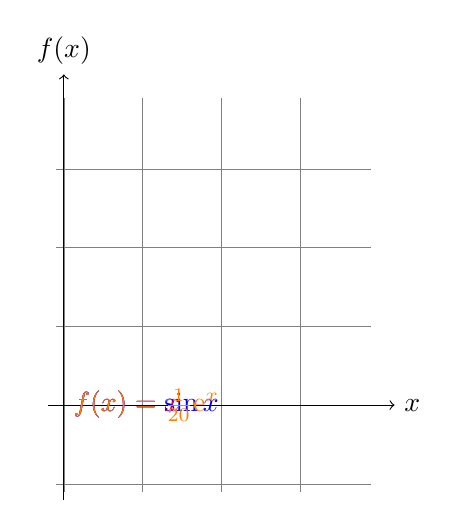
\begin{tikzpicture}[domain=0:4]
		\draw[very thin,color=gray] (-0.1,-1.1) grid (3.9,3.9);
		\draw[->] (-0.2,0) -- (4.2,0) node[right] {$x$};
		\draw[->] (0,-1.2) -- (0,4.2) node[above] {$f(x)$};
		\draw[color=red] plot[id=x] function{x} node[right] {$f(x) =x$};
		\draw[color=blue] plot[id=sin] function{sin(x)} node[right] {$f(x) = \sin x$};
		\draw[color=orange] plot[id=exp] function{0.05*exp(x)} node[right] {$f(x) = \frac{1}{20} \mathrm e^x$};
	\end{tikzpicture}

\end{document}


